\renewcommand\chapname{Hypertext for Nunggubuyu}
\renewcommand\longchapname{Language description and hypertext: Nunggubuyu as a case study}
\renewcommand\shortauthor{Simon Musgrave and  Nick Thieberger}
\renewcommand\longauthor{Simon Musgrave$^\spadesuit$ , Nick Thieberger$^\heartsuit$ \\
$^\spadesuit$Monash University, $^\heartsuit$University of Melbourne}
\chapter*{\longchapname}
\chapterauthor{\longauthor}
\mytoc{}


\begin{abstract}

Any reasonably complete description of a language is a complex object, typically composed of a grammar, a dictionary, and a text collection with internal relationships that can be represented as hyperlinks. The information would be fully searchable, links between text and media could be implemented, and the presentation would be based on a well-defined data structure with advantages for archiving and reusability. 

We present a small fragment from Heath's Nunggubuyu text collection with links to parts of the other elements of the description to demonstrate the benefit which this approach can bring. This initial step involves a certain amount of hand-coding but establishes a basis for the necessary data structure which will then be used in a second phase where we develop techniques for the automatic processing of scanned versions of Heath's work. 

Grammatical descriptions written with the kinds of structure we are developing, or capable of being converted to that structure (while being `born digital') are likely to be in short supply. Presentations of old materials in new formats will inform new electronic grammars, and help gain the acceptance of the linguistic community for preferred formats.

\end{abstract}


\section{Introduction}\label{thie:sec:1}
Any reasonably complete description of a language is a complex object. Traditionally, such works are divided into various components: a grammar, a dictionary and a text collection, the so-called Boasian trilogy. But of course these are really highly inter-related. For example, a single entry in the dictionary is of little value without the general information about words of that class which can be found in the grammar, and any point made in the grammar may be hard to grasp without extensive exemplification from texts. Boas himself was well aware of this fact:

\begin{quote}
  We have vocabularies; but, excepting the old missionary grammars, there is very little systematic work. Even where we have grammars, we have no bodies of aboriginal texts {\dots}. [I]t has become more and more evident that large masses of text are needed to elucidate the structure of the languages \citep[1]{Boas1917}
\end{quote}

As \citet[163]{Woodbury2011} comments on this passage: ``All three were interrelated parts of a documentary whole, treating, in different ways, overlapping empirical domains''.

The interrelatedness of the various components discussed above immediately suggests that hypertext would be a better means of presentation and additional benefits could come from making the grammatical description a multimedia object, rather than a text object. Examples could be heard in the original sound recorded by the researcher, or even seen as video clips where such presentation would aid the consumer (for example, where gesture added an important element of meaning to the utterance). In addition to the improved accessibility of the descriptive information, such presentation would bring the consumer much closer to the primary data, actual language in use, and therefore multimedia language description would increase substantially the standard of accountability in linguistics. However, the standard paper and ink presentation of grammatical description has an established linear format which is not suitable for the new medium. 

Most grammatical descriptions published in book format follow more or less closely a standard format. The presentation begins with background information on the language and its speakers, the relationship of the language to other languages, and a survey of previous research. The description proper then follows, moving through phonetics and phonology (the sounds of the language and how they are organized into a system), morphology (word-formation processes), and clausal syntax. Some discussion of syntax above the level of the individual clause and of textual organization may follow. If example texts are included in the volume, as is common, they will come after this, with word lists after them \citep{Nordhofftv}. The organization of a grammar in this style is linear, that is, one sort of information is presented before another. And the linearity is to a large extent well-motivated. It is generally not easy to understand the morphological processes of a language before one understands the phonology; it is hard to understand syntax (combinations of words) before one understands morphology (word-formation). Linearity of presentation is also a consequence of the medium. Paper and ink objects are read normally in sequence; even if one reads only a short section of a larger work, one starts at a particular place and reads on in sequence for as long as necessary. Hypertext, on the other hand, is a non-linear medium and the metaphor of a web is entirely appropriate for such presentation. As already mentioned, hypertext has clear benefits for the presentation of grammatical description, but it is desirable that at least some of the linear logic of the paper and ink model should be accessible in the new medium.

We wish to explore the possibilities of presenting grammatical description in an electronic form while maintaining a strong link with the traditional mode of presentation (cf Drude this volume). In order to do this, the ideal material to work with is a description presented in book format which nevertheless makes extensive use already of the interrelatedness of its various components. Jeffrey Heath's description of Nunngubuyu fits these criteria. The following section briefly describes this work and illustrates its value as an exemplar for developing richly interlinked language description for electronic presentation. Section~3 of this paper discusses our approach to encoding the source texts to make them accessible for online presentation and section~4 outlines our plans for further development of this project. Finally, in section~5, we turn to some design issues in electronic grammaticography as we view them in light of our work on Nunggubuyu. 

\section{Heath's Description of Nunggubuyu}
Nunggubuyu (ISO639-3: \texttt{nuy}, also known as Wubuy) is a non-Pama Nyungan language spoken in Arnhem Land, Australia (see Figure \ref{thi:fig:map1}).

\begin{figure} 
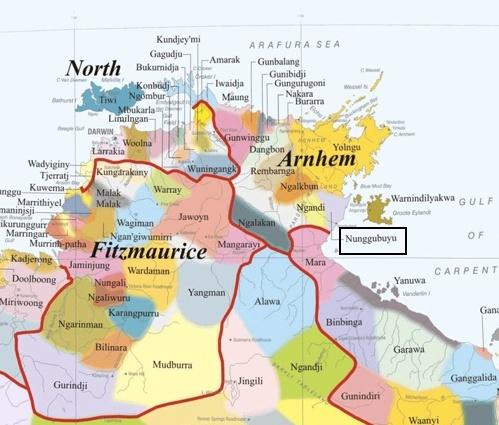
\includegraphics[width=\textwidth]{\imgpath/Thieberger2-img1.jpg}
\caption{Arnhem Land, showing the location of Nunggubuyu} 
\label{thi:fig:map1}
\end{figure}

Heath's description of the language was published in three volumes: texts \citep{Heath1980}, dictionary \citep{Heath1982} and grammar \citep{Heath1984}. The three volumes are very explicitly interlinked: the grammar volume does not include examples sentences, but a list of references to the text volume is given with each grammatical point and a similar procedure is followed in the dictionary (see Figure 1). The dictionary entry which is given in Figure \ref{thi:fig:fig1}\ref{thi:fig:fig1a} refers to Text 43, section 4, line 1 as an example of the lexeme in question. This section of text is given in Figure \ref{thi:fig:fig1}\ref{thi:fig:fig1b}, and the relevant word form can be seen in the first line. Figure \ref{thi:fig:fig1}\ref{thi:fig:fig1c} shows an excerpt from the grammar volume. From the fourth line of the excerpt, a list of text references which illustrate the point described is given; the fourth of these references (at the start of line 5) refers to the text fragment in \ref{thi:fig:fig1}\ref{thi:fig:fig1b} (43.4.3) and the relevant words can be seen in the third line of text.

\begin{figure}  
\subfigure[Dictionary entry from \citet{Heath1982}]{
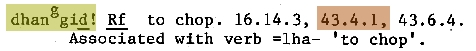
\includegraphics[width=\textwidth]{\imgpath/Thieberger2-img2.jpg}
\label{thi:fig:fig1a}
}
\subfigure[Excerpt from \citet{Heath1980}]{
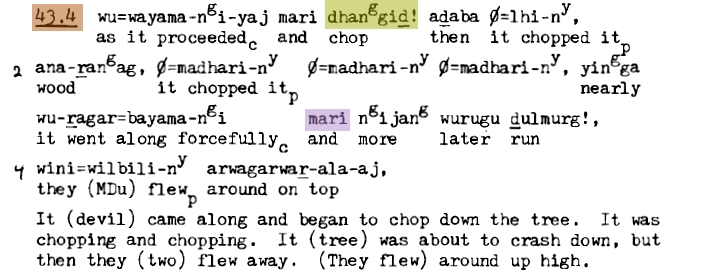
\includegraphics[width=\textwidth]{\imgpath/Thieberger2-img3.jpg}
\label{thi:fig:fig1b}
} 
\subfigure[Excerpt from \citet{Heath1984}]{
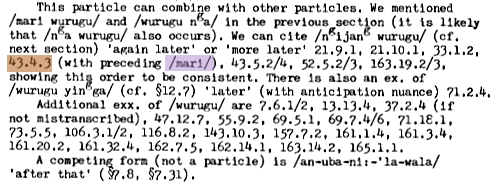
\includegraphics[width=\textwidth]{\imgpath/Thieberger2-img4.jpg}
\label{thi:fig:fig1c}
} 
\caption{Examples of linking between Heath's volumes} 
\label{thi:fig:fig1}
\end{figure}

The reader should bear in mind that we have carefully extracted these relevant sections from three separate books; in order to follow Heath's description to this level of detail requires manipulating and navigating three discrete physical objects.

Heath was very clear in his intention in following this practice. He emphasised in the introduction to the grammar volume that he was concerned with documentation: 

\begin{quote}
 These textual citations serve several purposes. When attached to a fully cited Nunggubuyu ex[ample], they have basically a documentary value -- the reader is assured that the ex[ample] is from a real text, and a reader wanting to know more or having doubts about the analysis can find it and analyse it.  [{\dots}] In this way, we take maximal advantage of the published texts (especially NMET*) achieving a far higher level of documentation than is observable in other reference grammars.'' \citep[4]{Heath1984} (*NMET = Heath 1980)
\end{quote}

And with accountability (see also Maxwell, this volume):

\begin{quote} 
 My concern with documentation reflects my own sad experiences as a reader of other linguists' grammars, which have almost never provided me with the information I wanted to undertake my own (re-) analysis of the language in question. It also reflects my experience that most published grammars are based on material obtained in unreliable direct-elicitation (sentence-translation) sessions [{\dots}] I have no confidence whatever in such data, since my own early `data' of this type often turn out to be seriously wrong. \citep[5]{Heath1984}
\end{quote}

However, these aims came at a price in terms of useability. In the course of otherwise extremely positive comments, two reviewers drew attention to the complexity of the work:
\begin{quote}
 ``Unfortunately, F[unctional] G[rammar of] N[unggubuyu] is a very demanding work, both because of the inherent complexity of the language and because it requires the reader to make constant reference to the text volume.'' \citep[310]{Blake1985} 
\end{quote}

\begin{quote}
 ``the work is particularly difficult to read. H[eath] makes no pedagogical concessions to the reader. One must look up the attestations for every major grammatical point in another volume.'' \citep[654-655]{Haiman1986}
\end{quote}

The linking structure which Heath included as an essential element of his description of Nunggubuyu lends itself naturally to treatment as hypertext links between documents,\footnote{The 
 fact that Heath's original recordings from his fieldwork are archived accessibly at the Australian Institute of Aboriginal and Torres Strait Islander Studies is an additional factor in our decision to work with this description.
} 
and we suggest it can serve as a first model for the structure of grammatical description in this format. For this model to be usable with new language data, it is necessary to establish encodings which, on the one hand, can be easily transformed into presentation formats while, on the other hand, still being formats with which linguists can work.

\section{Encoding issues}\label{thie:sec:3}
\subsection{Orthography }\label{thie:sec:3-1}
Heath uses a practical orthography to represent Nunngubuyu. This includes digraphs \graphem{n\textsuperscript{y}} and \graphem{n\textsuperscript{g}} to represent palatal and velar nasals respectively, and underlining of \graphem{t,d,r} to represent retroflex consonants. This system differs slightly from the system favoured by the speaker community today.
Our aim is to preserve Heath's orthography and to use transformations
to produce output in the current orthography where this is required.
As Unicode does not treat underlined characters as unique glyphs, in
basic formats we treat retroflex consonants as sequences of an
underscore followed by the relevant character (which can be rendered
by U+0331, the 'combining macron below' when necessary).


\subsection{Interlinear Glossed Text (IGT)}\label{thie:sec:3-2}
IGT is a common and extremely useful representation of bilingual text, capturing the complexity of the structural elements in the focus language in a morphemic level of annotation and providing a sentence-by-sentence translation at the free gloss level. Despite its ubiquity in linguistic description and despite theoretical modelling of various kinds\footnote{including 
  \citet{BowEtAl2003}, 
  \citet{HughesEtAl2003},
  \citet{HellmuthEtAl2006},
  \citet{Schmidt2003},
  \citet{Jacobson2006}, 
  \citet{JacobsonEtAl2001}, and \citet{PalmerEtAl2007}.
}
there is still no standard format for IGT that we could adopt in this model of linked Nunggubuyu data. The most common tool for creating IGT is probably \textit{Toolbox} with the benefit of lookup functions that allow parts of a corpus to be linked to the lexicon, to concordances and to specific wordlists \citep[see e.g.,][]{Hirzel2001}. The successor to Toolbox, \textit{FieldWorks,} addresses issues of interlinking by use of an underlying database, with the possibility of export to XML which may capture the relationships, but, if so, it is not clear to us what the schema is that allows these relationships to be encoded in the text.

Typecraft\footnote{\url{http://typecraft.org}} 
is a system for presenting interlinear text online served from an underlying database and uses Mediawiki, as does  Nordhoff's 2008 GALOES\footnote{ \url{http://www.galoes.org/}} which constructs an interlinked grammatical description. While these are ways of representing IGT using XML, there is no standard schema that provides a means for creating and linking between instances of IGT. Thus, for example, the online database of interlinear text (ODIN\footnote{ \url{http://odin.linguistlist.org/}}) which searches the web for likely examples of IGT, has to infer what IGT may look like from the alignment of text over several lines. Inevitably, such an inferencing approach results in many false positives and the data needs to be manually screened before it can be deemed to be a true sample of IGT. With the adoption of a standard IGT format such examples could be identified by web services and permit the retrieval of all and only IGT examples. 

In the Heath example under discussion, we opted to use EOPAS\footnote{ \url{http://www.eopas.org/}} \citep{SchroeterEtAl2006} both because it is a proposed standard and because it is built to work with primary media (as discussed in the next section). EOPAS is designed to take files in formats commonly created in the course of analysis, for example Toolbox IGT with timecodes linking the text back to the primary media, which it then transcodes to its schema. It also transcodes the media to formats playable using HTML 5 and highlights the textual chunks as their timecode is reached. As each utterance in EOPAS is citable to the level of the morpheme we are able to link from external objects, in this case the grammar and dictionary, to and from the morphemic level of an EOPAS file, as can be seen in the online example.\footnote{\url{http://users.monash.edu.au/~smusgrav/Nunggubuyu/17.HTML}}

\subsection{Media}
In what could be considered an additional or fourth member of the `Boasian trilogy' the audio or video recordings resulting from most fieldwork provide the basis for transcriptions and subsequent analysis. Maintaining the connection between the media and the derived or secondary materials (using Himmelmann's 2012 terms), \nocite{Himmelmann2012} as discussed earlier for the other outputs of language documentation, is now easily achieved and is slowly being taken up by linguists. A primary requirement of the citation of such media is that it have persistent identification which is provided by lodging the data in a suitable repository. Some repositories allow the media to be played directly from the archival location, while others allow for derived versions of archival material to be housed in accessible locations. EOPAS, discussed above, displays synchronised IGT and media and can either play from existing media files or from files uploaded to the EOPAS server. We included the media for a single text in our current project and encoded the IGT in a format suitable to allow for an EOPAS representation.

\subsection{Lexicon}\label{thie:sec:3-4}
There are a number of encoding formats for lexica which have been proposed or are in use \citep[for a slightly dated summary, see][]{Maxwell2008}. We have considered three\footnote{We 
 preferred these three options over the TEI dictionary format (\url{http://www.tei-c.org/release/doc/tei-p5-doc/en/HTML/DI.HTML}) mainly due to their being more targeted on small bilingual dictionaries.
} of these in developing this project: the Lexical Markup Framework (LMF\footnote{ \url{http://www.lexicalmarkupframework.org/}}), the Open Language Interchange Format (OLIF\footnote{ \url{http://www.olif.net/}}) and the Lexical Interchange Format (LIFT\footnote{ \url{http://code.google.com/p/lift-standard/}}).

Both LMF and OLIF have emerged from the environment of natural language processing and computational linguistics, and as a result both have rather Eurocentric models of the categories relevant to lexical data. In the case of LMF, this is perhaps less problematic as the data categories are kept separate from the specification of the format \citep[16]{Maxwell2008}. However, neither of these formats intuitively maps to the models of the lexicon used by descriptive linguists. Therefore we have preferred to use the Lexicon Interchange Format (LIFT) developed by SIL as our encoding scheme for the lexicon \citep{Hosken2006}. This format is intended to provide a well-structured XMLversion of the type of lexicon commonly used by linguists working with the Toolbox software and its successor FLEX. These software tools are popular with descriptive linguists, and using an encoding which is close to their file formats has obvious advantages.\footnote{Heath's 
 work on Nunngubuyu predates the availability of Shoebox (the precursor of Toolbox). The Nunngubuyu dictionary does exist in electronic form, as a Filemaker database.
} 
LIFT is also explicitly an \textit{interchange} format and we expect that scripts will become available shortly to move lexical data between this format and other popular and well-supported formats, including LMF and OLIF.

Figure \ref{thi:fig:fig2} shows an example of a LIFT encoded lexicon entry. Note that the  \tag{example} elements in this entry consist only of a reference to a source. This follows exactly Heath's practice in his dictionary. For our purposes, what is important is that the source information stored as an attribute in that element can be accessed and parsed to create a hyperlink to the relevant section of text when the lexicon entry is transformed into an HTML page. The `source' attribute is given here as a reference that can later be converted into a persistent identifier or URI, depending on the context in which the documents are delivered.

\begin{figure}
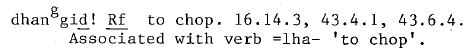
\includegraphics[width=\textwidth]{\imgpath/Thieberger2-img5.png}

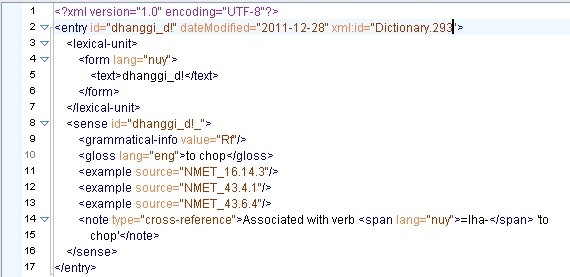
\includegraphics[width=\textwidth]{\imgpath/Thieberger2-img6.jpg}
\caption{Entry from \citet{Heath1982} with corresponding LIFT record} %
%This seems to be slightly inconsistent with the description and encoding below for the grammar: one would expect attributes like `source=``Text.16.14.3''~'.
%But indeed, given the possibility of interlinking arbitrary online resources, the ``source'' (and ``ref'') attributes should probably contain a more complete reference, ideally a PID (combined with an internal indication of the paragraph / entry / line etc.).
%
%NT {}-- I think these are fine and can be rendered as required by the next iteration of the program, as URIs or whatever. I've added a note to that effect above
\label{thi:fig:fig2}
\end{figure}

This entry also includes an identifier attribute in the  \tag{entry} element which is not a part of the LIFT format (\texttt{@xml:id}). This attribute is used for tracking references between the dictionary and other parts of the description; fuller discussion is presented in the following section. The numeric code is derived from the existing electronic version of the dictionary.

\subsection{Grammar}
We have already mentioned in section~1 that descriptive grammars have a more or less standard format. However, this format is a normative set of expectations about the order and means of presentation (see papers in \citet{EvansEtAl2006}, and in \citet{PayneEtAl2006}), rather than an accepted template, and it is therefore not surprising that no encoding for this document type exists. There are various kinds of encodings for grammars, including computationally tractable grammars (see also \citet[376]{Thieberger2009} on steps toward embedding a grammar in data), but we are here concerned with a marked-up textual encoding that permits interlinking. Our strategy in this example is to base our encoding on the Text Encoding Initiative Guidelines (TEI Consortium, no date) with additional elements as required.

The overall structure of the project requires that references from within the grammar to other parts of the description should be consistent in form and easily transformed to URLs which will point to relevant pages for online presentation. Heath's text already includes references to examples in the volume of texts and internal cross-references to other sections of the grammar. Although Heath does not include explicit links between the grammar and the dictionary, we wish to allow for such links in our version of the description. Such links are certainly implicit where Heath discusses specific lexical items within the grammar, and making the linking explicit is of great value as the language has considerable morphophonemic complexity which can make tracing lexical forms difficult. 

We encode all references with the TEI \tag{ref} element. This allows for the text representing the reference to appear in the document, thereby preserving the appearance of the original source. The location of the endpoint of a link is stored in the @target attribute of the  \tag{ref} element and takes the form of a pointer to the part of the description which is the target (Grammar, Dictionary or Text) followed by a numerical code. In the case of the grammar proper, the code matches the division shown in the table of contents and sub-heads; for example, chapter 7 sub-section 20 is coded as  \tag{ref target="Grammar.7.20"}. References to texts follow Heath's practice and specify the text identifier, a section number and a line number; for example a reference to line 2 of the third section of text 157 is encoded:  \tag{ref target="Text.157.3.2"}. The line numbering is an artefact of the original document; we have not yet encoded a large enough sample of the text collection to know whether this information will actually be useable in the web presentation or whether the interlinear presentation described in Section \ref{thie:sec:3-2} will rewrap texts in a way which makes this level of detail redundant. Retaining information from the source is of course best practice in this situation. References to the dictionary are to numerical codes which are an artefact of the existing electronic version of the material (FileMakerPro database); for example a reference to the lexical item \textit{i:-jung} is encoded:  \tag{ref target="Dictionary.4720"}. 

In all cases, the target material has to be coded with an identifier which exactly matches the originating pointer. This is done with an \texttt{@xml:id} attribute included in the relevant element of the different types of material. This coding has already been illustrated with the lexical entry example in Figure \ref{thi:fig:fig2}; similar attributes are attached to the  \tag{div} element which contains each section of the grammar and to the element  \tag{phrase} which holds each section of each text (and this can focus down to the level of  \tag{morpheme}). Figure \ref{thi:fig:fig3} is a section of grammar text with all three types of reference illustrated: line 57 includes a reference to the dictionary (created in our encoding), line 61 includes internal references to other parts of the grammar, and lines 78ff include references to text examples. 

\begin{sidewaysfigure} 
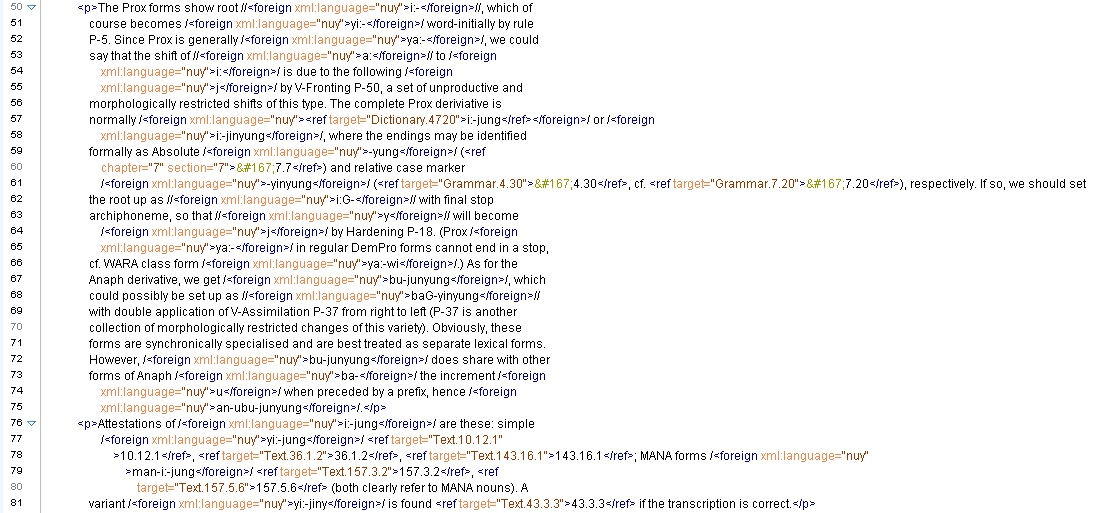
\includegraphics[width=\textwidth]{\imgpath/Thieberger2-img7.jpg}
\caption{Section of encoded grammar (from Heath 1984, section 7.25)}
\label{thi:fig:fig3}
\end{sidewaysfigure}


One additional type of reference occurs in the grammar, that is, citations of other works. The online presentation has a bibliography page, and citations are therefore encoded as pointers to items on that page. For example, a reference to Hore (1978) [1979]\footnote{Heath 
 1984 lists this work as Hore 1979; however the date of issue for volume 17 of \textit{Oceanic Linguistics} is 1978. Our internal reference retains Heath's error, but the Bibliography page includes a correction and clarification.
} \nocite{Hore1978}
is encoded as  \tag{ref target=``Bibliography.Hore.1979''}.

Figure \ref{thi:fig:fig3} also shows that we make extensive use of the TEI  \tag{foreign} element to encode words and phrases which are not English. In fact, all the examples of this element in figure \ref{thi:fig:fig3} enclose Nunggubuyu material, but in other places Heath includes cognate forms from other languages and the use of the \texttt{@xml:language} attribute is not redundant. 
 
\section{Further Development}
A small segment of the description of Nunggubuyu is available online at \url{http://users.monash.edu.au/~smusgrav/Nunggubuyu}. The XMLsource of these pages was hand-coded and HTML was then generated using search-and-replace in a text editor. Obviously, these procedures are time-consuming and, having established reasonably stable principles for encoding the material, our next priority is to automate the process as much as possible.

A first step in this endeavour will be to attempt to produce electronic versions of the original texts using optical character recognition software (OCR). As discussed in Section \ref{thie:sec:3-1}, Heath's texts use an idiosyncratic orthography with superscript characters which are important. The original text also uses subscript characters in gloss lines to indicate various grammatical properties. All of these characters will need to be captured by OCR if the process is to be useful. Even if OCR is successful at that level, it will still be necessary to use scripts to insert some appropriate encoding of the non-standard characters. It seems quite likely that the post-editing which will be needed to make an OCR version of the material useable may be so extensive as to render the whole process too slow. The alternative then would be to have the source materials retyped directly to our preferred encodings%
%See Michael Cysouw's dictionary project: he sends all his scanned material to (south)east Asia for re{}-typing and is content with both prices and results.
%
%Right, and we would potentially do that too, but it is not necessary to state it here.
; this would also be time-consuming (and expensive), but may be a more efficient alternative. If OCR turns out to be a viable means of generating a complete electronic version of the material, we would still need to develop scripts to add encoding to the basic text. This is still not a particularly attractive option as such scripts will be specific to the source with which we are working. If in the future we wished to import another pre-existing description to our format, we would almost certainly need to at least considerably modify the scripts used to add mark-up.

Various issues concerning the internal linking of the materials will arise when we are able to work with the entire description. As noted in Section \ref{thie:sec:3-4}, we believe that it will be useful to include  links explicitly which Heath left as implicit%
%Another case are the constant cross{}-references to RULES (such as P{}-5, P{}-50 etc. in Fig.~3), which should also correspond to  \tag{ref} elements.
, such as those pointing at rules (such as P-5, P-50 etc. in Figure \ref{thi:fig:fig3}) or between lexical forms in the grammar and corresponding dictionary entries and those between dictionary entries which are cross-referenced. Three questions will have to be addressed in generating such links. First, to what extent is it useful to make the implicit structure explicit? There are cases where doing so is clearly advantageous; in the following paragraph we discuss an instance where we have included a reverse link (from text to grammar) to complement the link Heath made between grammar and textual instance. But we can imagine that in some cases fully explicit linking might be counterproductive: will the user always want to have access to every textual instance of a common morpheme? It will be desirable to allow the possibility that a user can search for every instance, but listing every one with an explicit link would probably be unnecessary (See Good's (this volume, section 8.1) distinction between examples and exemplars{}---the latter being carefully selected to illustrate a point, while the former are more or less the harvested results of a search). %
%See Jeff Goods distinction between examples and exemplars {}-- the latter being selected by hand.
Second, how can this process be done automatically? This is only a problem for dictionary entries as references to texts and to sections of the grammar will always be in a form (numerical code) which can be parsed automatically. For the dictionary, however, we believe that it will be necessary to create a look-up table against which the texts and grammar can be compared to identify forms which should be linked to dictionary entries. The third question to be considered is whether the resulting structure should be implemented as simple hypertext links, or whether it will be more stable and efficient to use a link table (that is, a simple database) to store the links. Doing so will mean using some scripting language to actually implement the links, and this is not desirable; in principle, we would prefer to keep the whole implementation in HTML only. However, there are additional considerations, to which we now turn, which suggest that such an HTML only implementation will not be practical.

Even in the very small sample which we have produced so far, we have encountered a problem in realising the complexity of the links which allow the user to move from one part of the description to another. In the text sample online, we have linked some forms to their dictionary entries; this has been implemented at the morphemic level of the text. But there is one case (\textit{da:n} in line 1 of the text) where we have also implemented a link from this morpheme to a section of the grammar. This is a link which is only implied by Heath: the grammar refers to the text as a relevant example, but there is no annotation in the text to indicate the relevance of the grammar section. There are thus two targets linked from a single source morpheme at this point. We have dealt with this by instantiating the link to the dictionary on the morphemic analysis line and the link to the grammar on the text line, and this is an adequate solution in this case. However, we are aware that there will certainly be cases where a single form in a text will need to be linked to more than two targets. For example, a motion verb form might be linked to a description of the class of verbs to which it belongs, to an analysis of the morphophonemic changes which the form undergoes as well as to a discussion of how directionality is treated in the language. With a link to the dictionary as well, this will require four links to be instantiated from only two source forms, which is not possible using HTML only. We suspect that we will want to use a technique such as menus which pop-up when the cursor is over a form in order to handle this sort of complexity. We also suspect that, when the full complex structure of links is created, the actual appearance of texts on the screen will be problematic. Every form, or almost every form, will be the source of a link. 
If these links are simple HTML links, then (almost) every form will
be a link, making it difficult to visually distinguish links from
non-links in the text. This is  problem that we expect to be able to
deal with using style-sheets in the delivery version. If we need to use some programming resources to handle multiple links from a single source, then it will probably be worth also using such resources to implement links to the dictionary with keystrokes. For example, selecting a form on the morphemic tier and using the keys \texttt{Alt+D} would take the user to the relevant dictionary entry in every case. We also anticipate that there will be problems to solve for links to grammar sections which discuss constructions rather than individual forms. It is not immediately clear whether the source of such links should be individual words or morphemes, or the entire span of text which is relevant. 

The various questions just raised will become relevant when we have all of the description encoded and potentially available as hypertext. At that point, we expect to have to make decisions about how to deal with the problems and this will most likely mean making a decision about a programming or scripting language to use to develop the online environment which we want. 

A further and critical matter to be confronted in the creation of any data is the longevity of the material created. As stated earlier, one motivation for encoding a grammatical description is explicitly to allow the rich set of links implicit in a grammar to be stated and stored as text, a preferred archival format. Persistence of the primary media and any secondary analysis would, as a matter of course, be provided by an appropriate repository and the links between objects described here would resolve to these archival forms or derived versions (as HTML, or streaming media for example) in suitable locations. Although we have introduced the possibility that delivery in a browser will require resources beyond those offered by (current versions of) HTML, our approach ensures that the linking structure is explicitly encoded in archival data sources. Optimal presentation may depend on particular implementations, but presentation is independent of the basic data. We note that in the case where the data is not derived from printed material, this means that a rendering as a printed object will also be easily achieved.

\section{Designing Electronic Grammaticography}
Electronic grammaticography is the topic of all chapters in the present volume, and also of \citet{Good2004}, \citet{Nordhoff2008}, and \citet{BenderEtAl2004}. Our project is offered as an example both of retrofitting an existing grammatical description and of setting out what requirements more elaborated grammar-template projects could include. We have described here the preliminary stages of a project which aims to make a classic grammatical description available as an electronic resource. We have discussed a number of problems which arise in transferring such material from its original form as printed text to a new format which makes new and richer possibilities available, and the reader might be tempted to ask whether there is any point to grappling with such problems; might it not be simpler to work with newly-produced materials which are already available in electronic formats? Obviously, we believe that the effort is worthwhile, and we would like to close by offering some of our reasons for this view and showing how they relate to basic issues in the development of electronic grammaticography.

First, most of the problems we have discussed in Section \ref{thie:sec:3} are about choosing suitable formats and encodings for source material. Most of these problems would still need to be faced in working with recent materials. Many linguists work with texts and lexicon in Toolbox, but this practice is not universal, and even those who do structure their files differently. Even for material originating in Toolbox, decisions would need to be made about a common encoding to be used as an interchange on the way to online presentation, and such an encoding would also have to be used for materials from other source software. Although the practical problems of transferring material from one format to another would be simpler for description born digital, the conceptual issues would be the same. And for actual grammatical description, the range of formats used by different scholars would be considerable; again the conceptual issues are the same as those we have discussed. (If we are able to present grammatical description online in a useful and attractive way, we would hope that other scholars might then adopt our encoding practices, but we are not aiming to impose a standard on our colleagues, only to find a pragmatic solution.)

Second, we believe that it is important to be able to handle grammatical description which already exists as legacy materials. The advantages which we see for the mode of presentation discussed in Section \ref{thie:sec:1} are considerable. Assuming that we can achieve the aims which we have set out here, we believe that it will be very desirable to make as broad a range of grammatical materials as possible available in this way. 

Third, and following from this previous point, we believe that the design of electronic grammaticography should incorporate the best practice of traditional grammaticography and then extend it. Heath's work is an ideal starting point for this endeavour. As we discussed, Heath had a carefully considered view of how the parts of his description should interact for the user. The format which was available to him made this very difficult in practice but we can now attempt to implement that interactivity in a more congenial format. Even replicating what Heath included in his work means addressing fundamental questions about how electronic grammaticography can work. Going beyond Heath and making the web of interconnections more complete and more explicit poses additional problems. We suggest that adequate solutions to these problems will provide a sound basis for one version of electronic grammaticography. 

